\chapter{Contribution}

Definition of Binder et al. \cite{binder_definitions_2022} is promising, however the branch prediction and the related issues are not taken in account by the framework. Thus we aim to extend the use case of proposed definition.

In our work we try to adjust Binder's definition to the setting of pipeline with branch predictor. We introduce an input format capable of expressing speculative execution. 

\TODO{complete intro when chapter is done}

\section{Methodology}

\subsection{Existing framework overview}

\subsubsection{Exploration by model checking}

The implementation provided by Binder is written in TLA$^+$ \cite{lamport_specifying_2003}. The pipeline state is specified in set-theory notation. The model checker step corresponds to a one clock cycle and derives a new HW state from the previous one. This allows to simulate the non-deterministic timing behavior: each time when a variation can happen, multiple next state are generated. TLA$^+$ covers all reachable states ensuring that all possible behaviors are covered.

The pair of trace constitutes a whole model state. TA is expressed as an invariant for the pair of traces, so its is verified in each model checking step. 

As well as a construction of traces, the framework provides visualization methods for the traces and ETDG.

\TODO{each pair of executions is considered? or all executions are compared against the one reference?}

\subsubsection{Input trace format}

The input of the framework is a pair of:
\begin{enumerate}
	\item Pipeline parameters: superscalar degree, $FU$ latencies and memory access latencies depending on the cache events (hit or miss). sequence of instructions;
	\item Instruction sequence: for each instruction its type and registers are specified as well as set of cache behaviors to be explored by the model checker. The type is used to know which $FU$ will be used by the instruction and based on registers data dependencies are retrieved.
\end{enumerate}

We can simplify this view by directly expressing the resource, dependencies and possible latencies of instruction. Figure \ref{fig:input-format} shows the input for instruction trace from example \ref{ex:simple-ta}. First column is instruction label, second is the resource used, thirds is the sep of data dependencies and the last one captures possible execution latencies. In the same fashion we could specify variations of latencies for $IF$ stage, but we skip them for simplicity. This format is sufficient to express a pair of execution traces derived from instruction trace.

\TODO{example of input in TLA}

\begin{figure}[htbp]
	\centering
	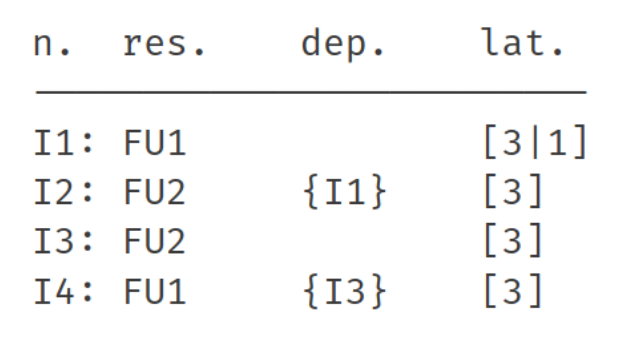
\includegraphics[width=0.3\textwidth]{figures/input_ex.png}
	\caption{Simplified input format of example from figure \ref{fig:TA1-code}}
	\label{fig:input-format}
\end{figure}

\subsection{Limitations}

Despite using a model checker, the existing framework is capable to explore only the traces that fit the instruction template. This limits the explored space to what is manually defined by the user. Considering that branches are to be added, this limitation is becoming even more restricting. 

Nevertheless, the framework may be used to manually specify the instruction trace using a template and generate a resulting pair execution traces. This allows to quickly sketch the examples and analyze them. Unfortunately this feature comes up with some issues.

The significant flaw we noticed was the performance. Firstly, the TLA$^+$ itself takes a few seconds to generate initial states of the model. Secondly, the graph is analyzed using java embedding which calls a script in python which in its turn deserializes a graph from text output of the model checker tool. 

Moreover, the input is specified in lengthy TLA$+$ notation, which prevents fast sketching the examples. Thus it was decided not to write an extension of the existing framework, but to design a new one from scratch.

\subsection{Our novel framework}

c++

3 modes of using: manual, random, total

\subsubsection{Supporting Speculative Execution in Input Format}

\section{Adapting definition of Binder et al.}



\section{Gap problem}

\section{Formal Requirements for Causality Graph}

\section{New Causality Definition}

\section{Taking BP state into account}
Put to conclusion?

\section{Results}

put examples of different TA here